\section{Results and Discussion}
\label{sec:results}

Many numerical experiments were conducted to validate the \Cyder software library.
Multi-component simulations demonstrated expected transport behavior and
the successful collective interaction of the modular
components in a \Cyder repository. Single-parameter sensitivity analyses
demonstrated that physics captured by the \Cyder models compare favorably to
results reported in \cite{huff_key_2012} from a more detailed existing model,
the Clay \gls{GDSM}, developed by the \gls{UFD} Campaign within the
\gls{DOE} Office of Nuclear Energy \cite{clayton_generic_2011}.

In addition to these numerical experiments, a robust unit test suite was
deployed during development to verify \Cyder software implementation.

\subsection{Multi-component Simulations}
% Many numerical experiments were conducted to verify and validate this code.

% The interaction between components is demonstrated by an example simulation

%Also, for most of 5.2, you need to make the case that the single result you show
%is representative!!  I think that's easy, but needs to be done.  Essentially,
%you need to make the case that for real isotopes, the same model will be
%invoked with real parameters, so that these normalized (relative?) parameters
%are representative of all cases.

To verify the fundamental behavior of all four \Cyder radionuclide transport models at
each component interface, many transport and containment base cases were
conducted.

The simulations were conducted within the \Cyclus framework and had the
following simulation parameters:

\begin{itemize}
\item{A 1000 year simulation}
\item{A source facility providing one waste stream per time step}
\item{An initial capacity of five 1 kg waste streams (in most cases)}
\item{No more than one waste stream object is stored per waste form}
\item{Corresponding waste package components, one per waste form}
\item{A buffer component (i.e. a bentonite clay)}
\item{A far field component (i.e. the host rock)}
\end{itemize}


Each feasible combination of the four models was conducted to verify
implementation of the time stepping algorithm and transport modes between
components. A full description of each of these verification simulations can be 
found in the dissertation \cite{huff_integrated_2013}. Among these simulations, 
one in which each component is represented with a Mixed Cell model is shown 
in Figures 
\ref{fig:mcIIIall} through \ref{fig:mcIII}.  
The fixed maximum transport mode was used between mixed cell components for speed and clarity of results.

Solubility limitation is enabled 
in this case, so the system is expected to demonstrate solubility limited 
transport.  To simultaneously demonstrate the behavior of the solubility 
limitation, no sorption is applied, but solubility limitation is set to 0.001 
kg/m$^3$ for all isotopes.  Please note that the \Cyder user must currently 
provide reference solubility values for each isotope. While this offers the 
user complete control, it may be inconvenient for some users. Future extensions 
to \Cyder will include a default database for these values, perhaps through the 
\gls{PyNE} database toolkit\cite{bates_pyne_2014}. 


\begin{figure}[ht]
\centering
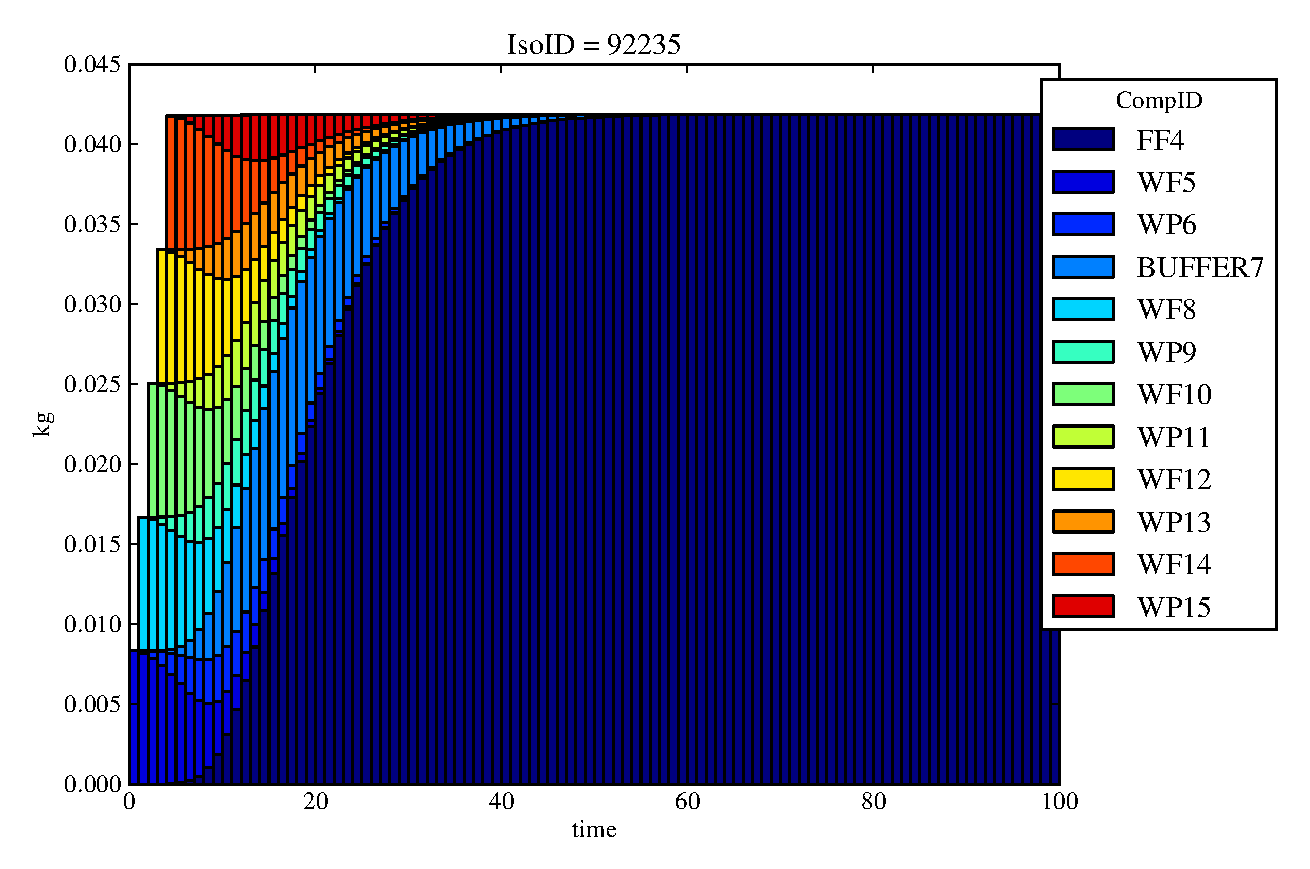
\includegraphics[width=0.6\textwidth]{./results/images/mcIII.eps}
\caption[$^{235}U$ residence. Mixed Cell Coupled Sorption and Solubility Limitation.]{
For the MCIII case in which containment is affected by solubility limitation,
        ($F_{d}=0.1$ for all components except far field), $^{235}U$ travels through waste 
        packages (WPN), their corresponding waste forms (WFN), and the surrounding 
        buffer (BUFFER7) more slowly than in the MCI case
        before permanent residence in the far field component (FF).
}
\label{fig:mcIIIall}
\end{figure}

\begin{figure}[ht]
\centering
  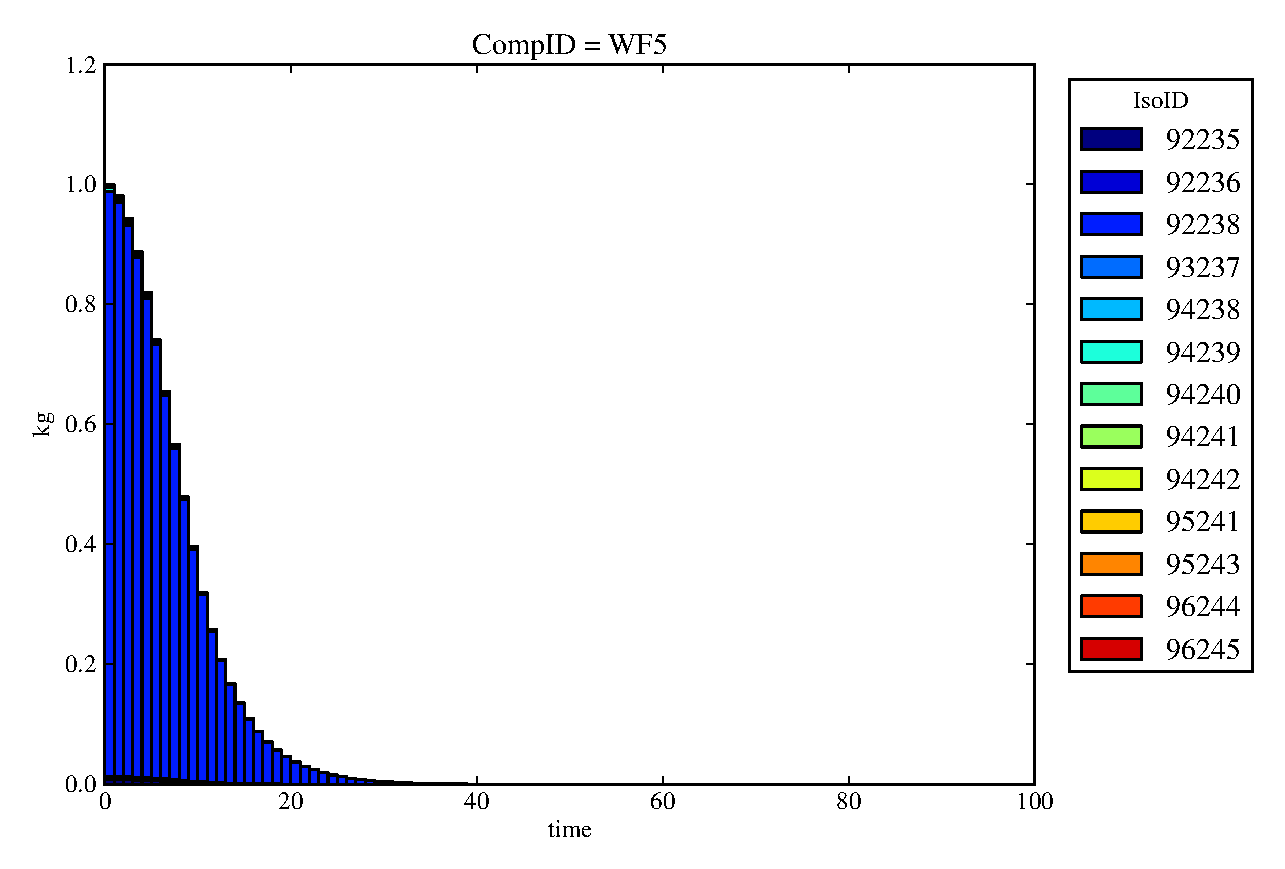
\includegraphics[width=0.6\textwidth]{./results/images/mcIII1.eps}
  \caption[Case MCIII Waste Form Contaminants.]{
          Waste Form 5 (degradation rate $F_d = 0.1[y^{-1}]$, reference solubility limit $S_{ref} = 0.001kg/m^3$) releases material with degradation.
    }
  \label{fig:mcIIIwf5}
\end{figure}


\begin{figure}[ht]
\centering
  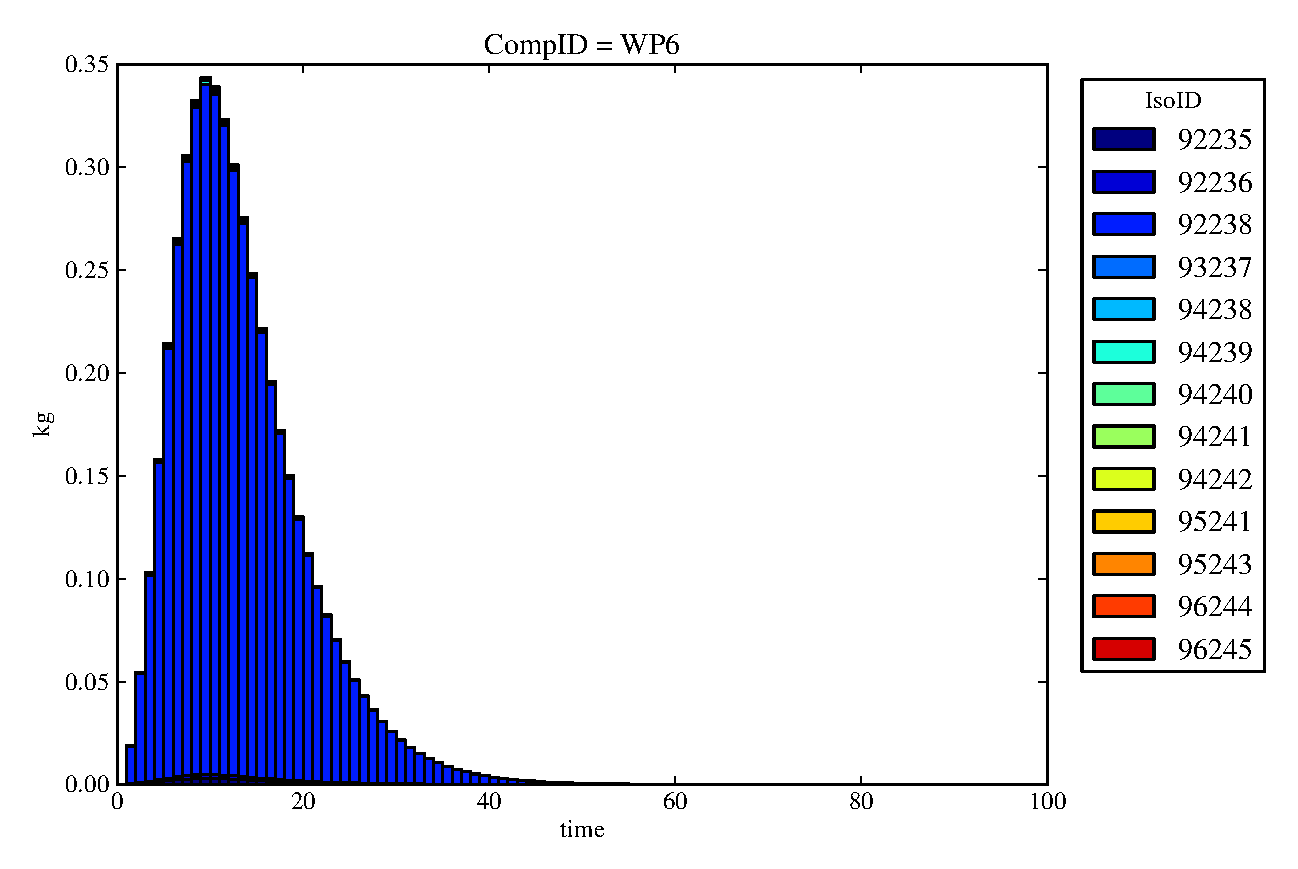
\includegraphics[width=0.6\textwidth]{./results/images/mcIII2.eps}
  \caption[Case MCIII Waste Package Contaminants.]{
          Waste Package 6 (degradation rate $F_d = 0.1[y^{-1}]$, reference solubility limit $S_{ref}=0.001kg/m^3$) receives then releases material.
    }
  \label{fig:mcIIIwp6}
\end{figure}

\begin{figure}[ht]
\centering
  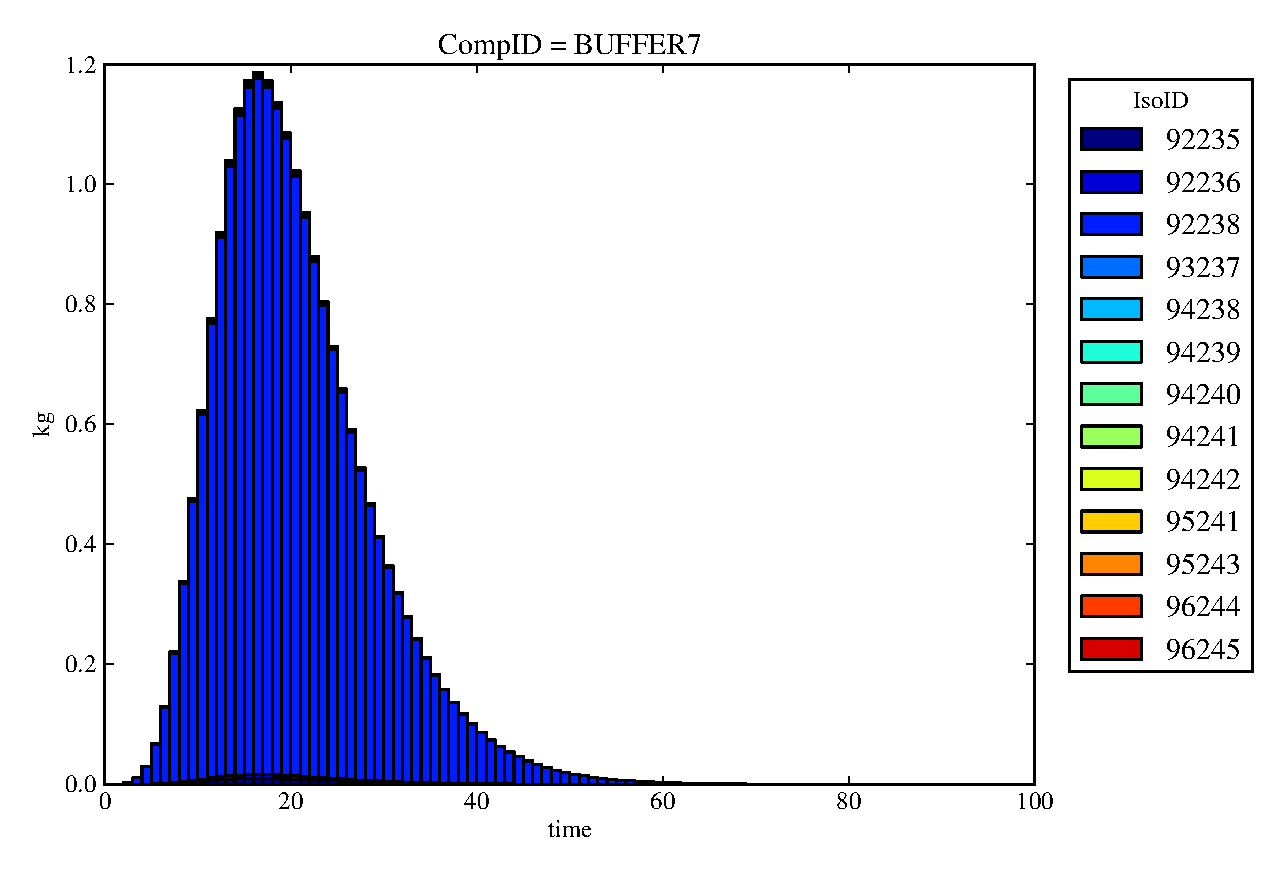
\includegraphics[width=0.6\textwidth]{./results/images/mcIII3.eps}
  \caption[Case MCIII Buffer Contaminants]{
          The Buffer, component 7 (degradation rate $F_d=0.1[y^{-1}]$, reference solubility 
        limit $S_{ref}=0.001kg/m^3$), receives and then releases material.
    }
  \label{fig:mcIIIbuff}
\end{figure}

\begin{figure}[ht]
\centering
  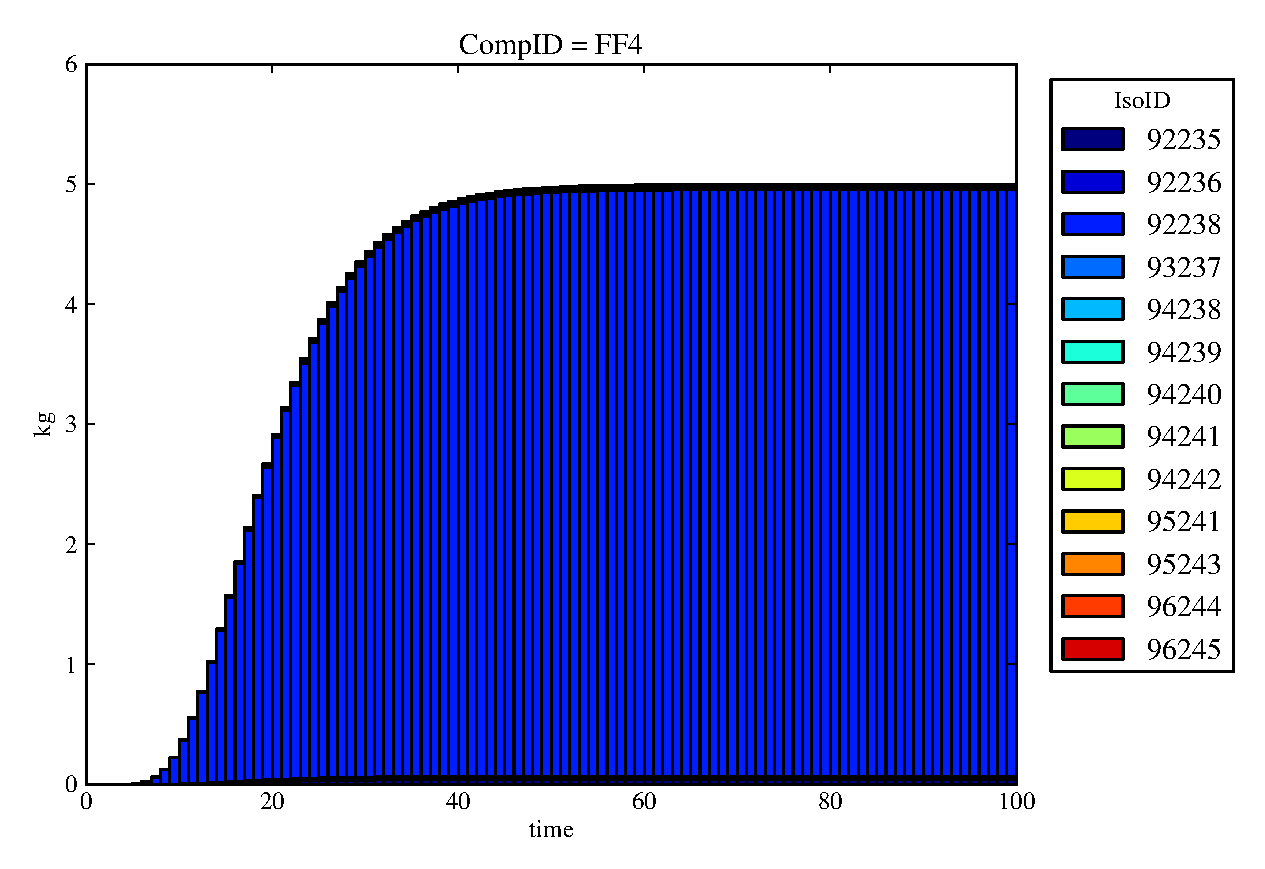
\includegraphics[width=0.6\textwidth]{./results/images/mcIII0.eps}
  \caption[Case MCIII Far Field Contaminants.]{All material is released into
        the Far Field, component 4 (degradation rate $F_d=0.0[y^{-1}]$, reference solubility limit $S_{ref} = 0.001kg/m^3$).}
  \label{fig:mcIII}
\end{figure}



\FloatBarrier



\subsection{Single Effect Parametric Analyses}
% Many parametric analysis were conducted to validate system responses
\subsubsection{Solubility Sensitivity}
Each of the radionuclide contaminant transport models described in Section
\ref{sec:nuclide_models} capture different combintations of physics present in
the hydrologic contaminant transport problem. To determine how effectively
these physics were captured, single-effect simulations were conducted with
\Cyder and compared to analysis was conducted with a more detailed radionuclide
transport model, the Clay \gls{GDSM} \cite{clayton_generic_2011}. The Clay
\gls{GDSM} was developed by the \gls{UFD} Campaign within the \gls{DOE} Office
of Nuclear Energy and relies on the GoldSim simulation environment
\cite{golder_associates_goldsim_2010} and its contaminant transport module
\cite{golder_associates_goldsim_2010-1}.

These single-effect sensitivity analyses were constructed by repeated
multi-component simulation runs conducted accross the valid range for a single
parameter.

To verify the behavior of the solubility limitation model in the Mixed Cell
model, for example, one hundred multi-component simulations were conducted,
each with a different reference solubility limit. This parametric analysis was
conducted to show that, for an arbitrary isotope, the expected solubility
limitation behavior is captured. In the case of real isotopes in a full
simulation, the same model will be invoked with real parameters for each
isotope. Thus, the this model agreement is representative in all cases.

The results acheived with \Cyder were compared to the results of a parametric
sensitivity analysis using the Clay \gls{GDSM} reported in
\cite{huff_key_2012}. That analysis showed that for solubility limits below a
certain threshold, the dose releases were directly proportional to the
solubility limit, indicating that the radionuclide concentration saturated the
groundwater up to the solubility limit near the waste form.  For solubility
limits above the threshold, however, further increase to the limit had no
effect on the peak dose. This demonstrates the situation in which the
solubility limit is so high that even complete dissolution of the waste
inventory into the pore water is insufficient to reach the solubility limit.

\begin{figure}[ht]
\begin{center}
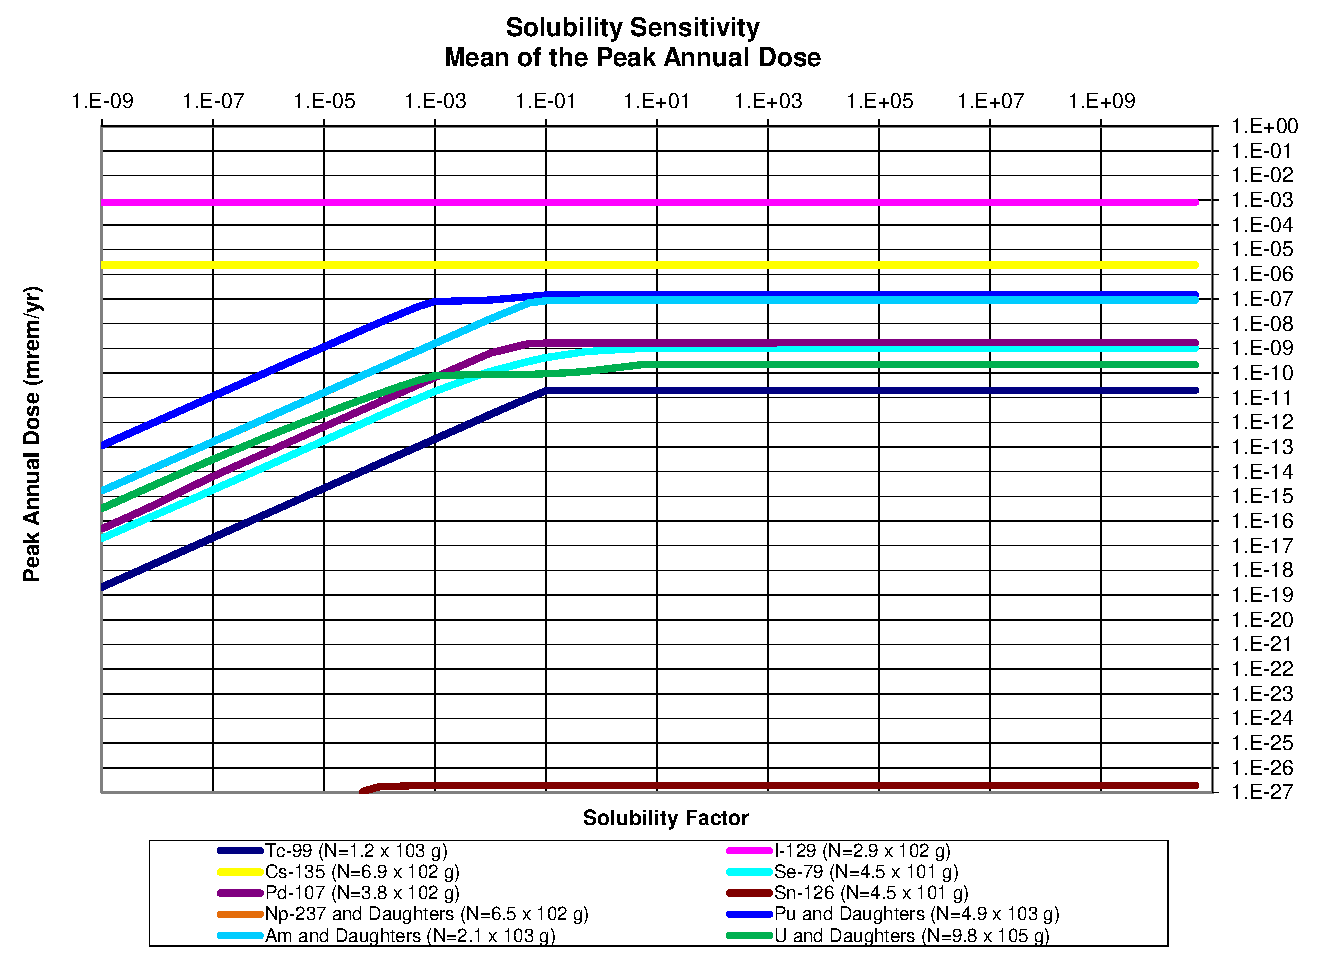
\includegraphics[width=0.7\linewidth]{./results/images/Solubility_Summary_SolFactor.eps}
\caption[Solubility factor sensitivity in GDSM Clay model]{Solubility factor sensitivity. The peak annual dose due to an inventory, $N$, of each isotope. This result was acheived with a parametric analysis using a detailed model of a generic clay repository \ref{huff_key_2012}}
\label{fig:SolSumFactor}
\end{center}
\end{figure}

\begin{figure}[ht]
\begin{center}
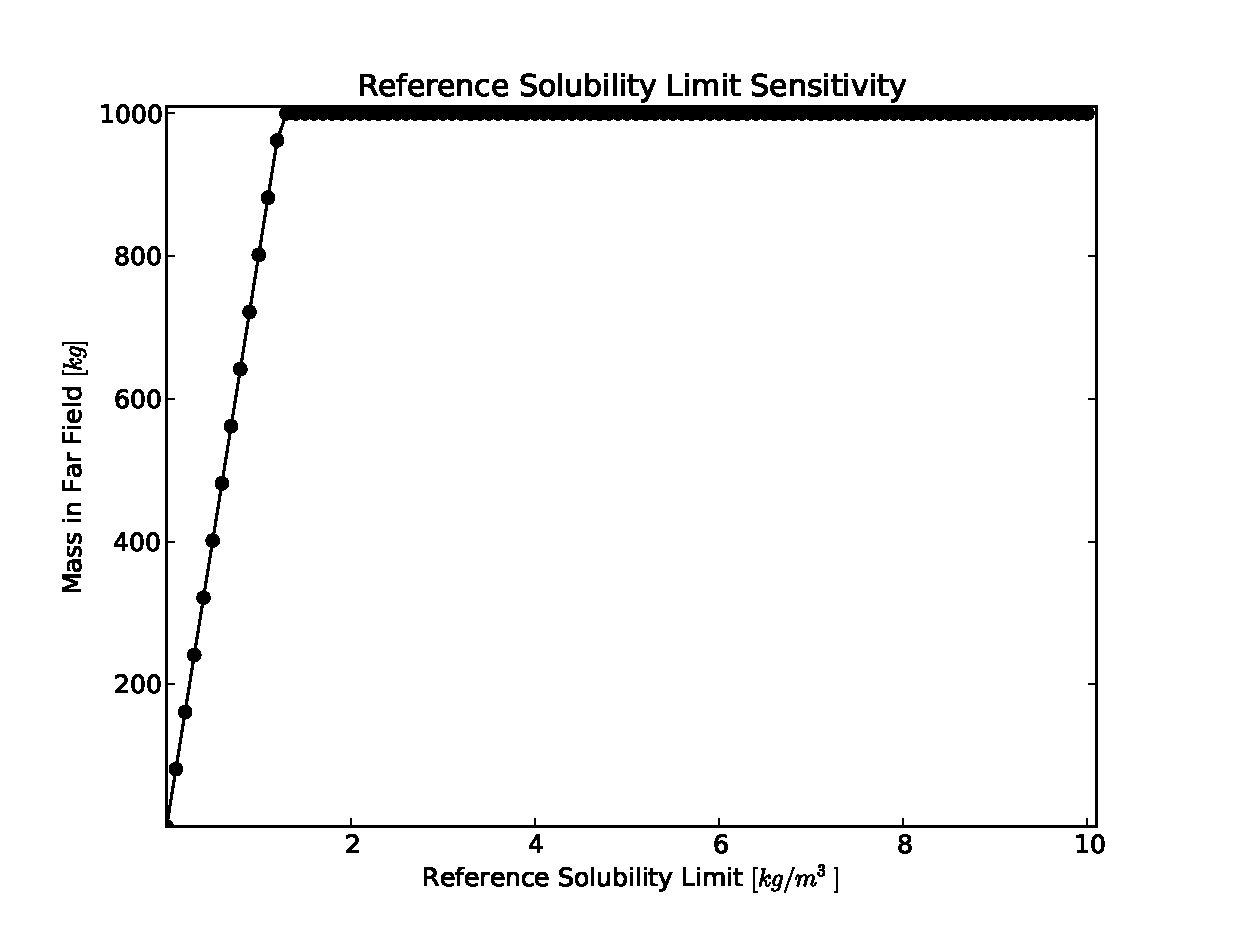
\includegraphics[width=0.7\linewidth]{./results/images/sol.eps}
\caption[Solubility Sensitivity in the Mixed Cell Model]{Sensitivity demonstration of solubility limitation in \Cyder for an arbitrary isotope assigned a variable solubility limit.}
\label{fig:sol_result}
\end{center}
\end{figure}


The results in Figure \ref{fig:SolSumFactor}, from the detailed parametric
analysis in \cite{huff_key_2012}, it is clear that for
solubility constants lower than the saturation threshold, the transport regime is solubility
limited and the relationship between peak annual dose and solubility limit is
strong.  Above the threshold, the transport regime is inventory limited
instead.

In the corresponding parametric analysis of \Cyder performance, it was shown that the
solubility sensitivity behavior closely matched that of the \gls{GDSM}
sensitivity behaviors. Specifically, in Figure \ref{fig:sol_result}, a sharp turnover
is seen where the solubility limit exceeds the point at which it limits
movement. For increased solubility limits, release remains constant, as
expected.

%\begin{figure}[ht]
%\begin{center}
%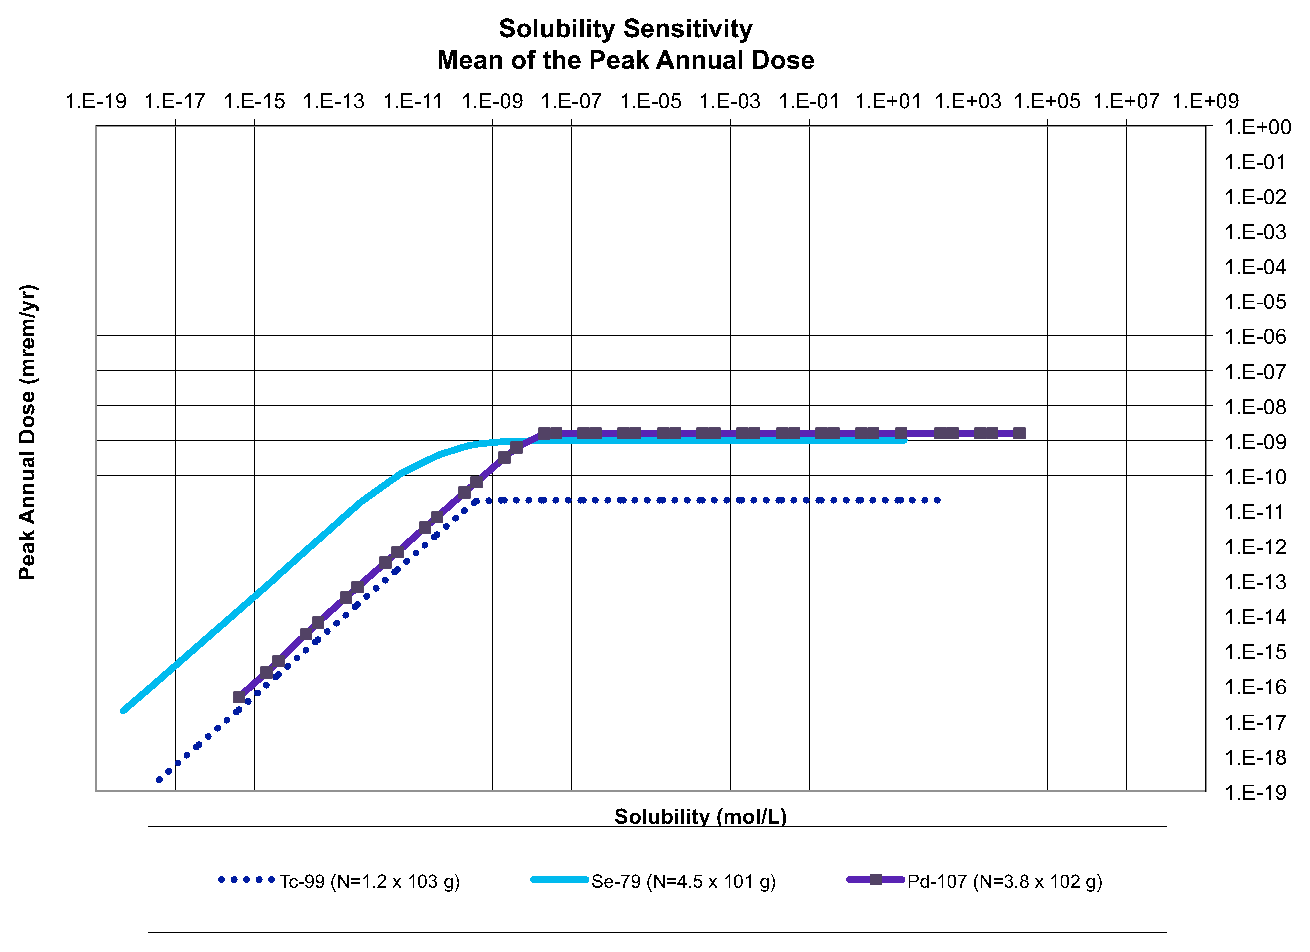
\includegraphics[width=0.7\linewidth]{./results/images/Solubility_Summary_Sol.eps}
%\caption[Solubility limit sensitivity in GDSM Clay model]{Solubility limit sensitivity. The peak annual dose due to an inventory,
%$N$, of each isotope.}
%\label{fig:SolSum}
%\end{center}
%\end{figure}


\FloatBarrier
\subsubsection{Sorption Sensitivity}



As the distribution coefficient $K_d$ increases, so does the retardation 
coeffcient $R_f$, according to the relation $R_f = 1+ \rho_b\frac{K_d}{\theta}$. As these two values increase, contaminants tend 
toward the solid phase. An increase in these coefficients, then, has the effect 
of limiting dissolved concentration.

In the parametric sensitivity analysis reported in \cite{huff_key_2012},
the expected inverse relationship between the retardation factor and resulting
peak annual dose was found for all elements except $^{129}I$ and $^{79}Se$. 
These two isotopes have effectively no solubility limit and therefore
demonstrate no sensitivity whatsoever to a the solubility limit multiplication 
factor. In the low retardation coefficient cases, a regime is established in 
which the peak annual dose is entirely unaffected by changes in retardation 
coefficient.

For large values of retardation coefficient, the sensitivity to small changes
in the retardation coefficient increases dramatically. In that sensitive
regime, the change in peak annual dose is inversely related to the retardation
coefficient. Between these two regimes was a transition regime, in which the
$K_d$ factor ranges from $1\times10^{-5}$ to $5\times10^{0} [-]$.

It is clear from Figure \ref{fig:KdSumFactor} that
for retardation coefficients greater than a threshold, the
relationship between peak annual dose and retardation coefficient is a strong
inverse one.

\begin{figure}[ht]
\centering
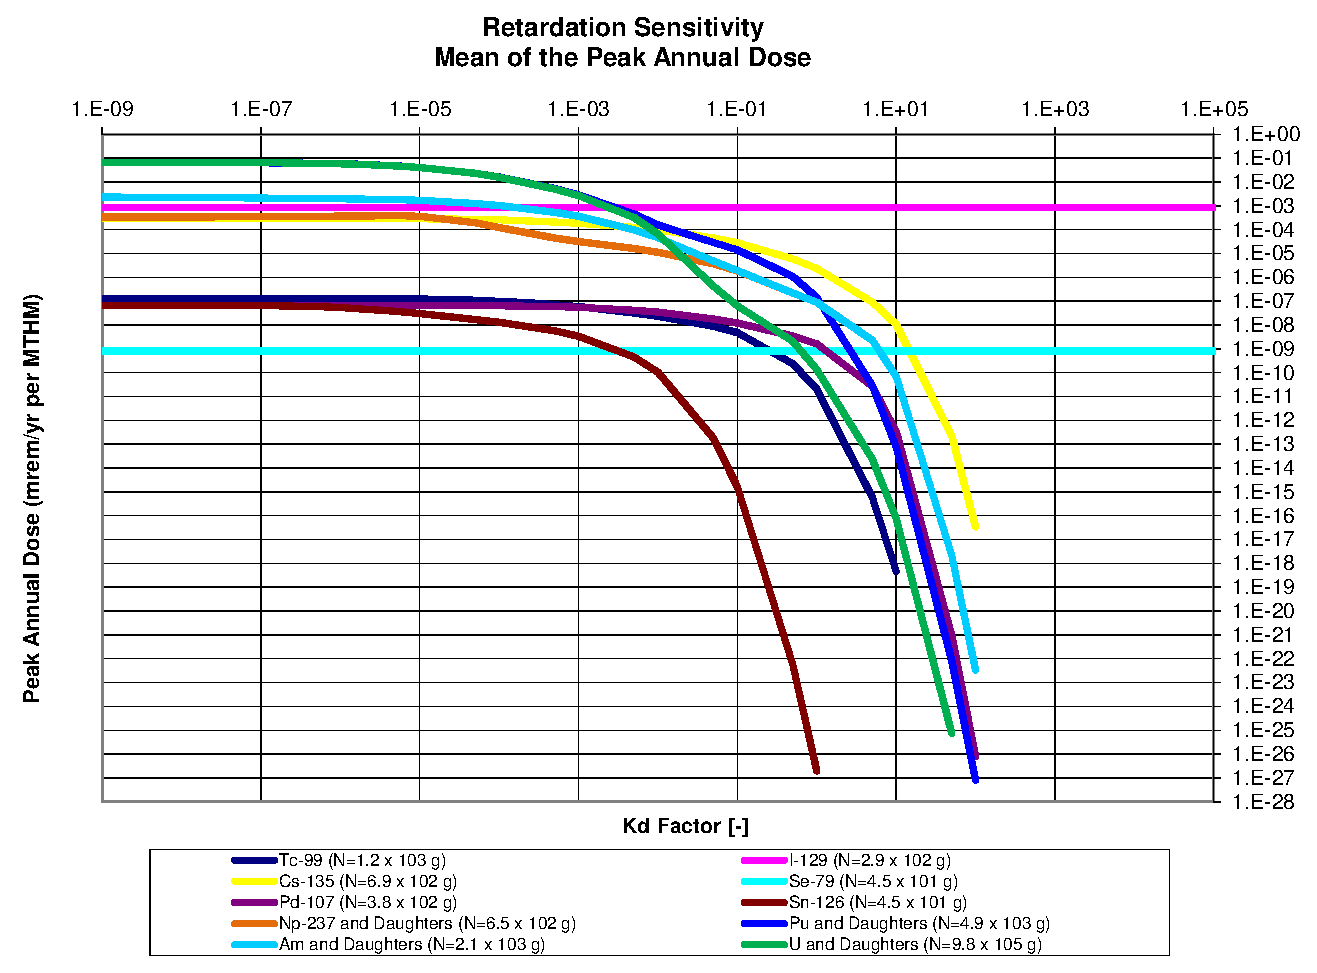
\includegraphics[width=0.7\linewidth]{./results/images/Retardation_Summary_kdFactor.eps}
\caption[$K_d$ factor sensitivity in Clay GDSM]{$K_d$ factor sensitivity in 
        DOE Clay GDSM, reproduced from \cite{huff_key_2012}.
The peak annual dose due to an inventory,
$N$, of each isotope.}
\label{fig:KdSumFactor}
\end{figure}

\FloatBarrier


In the parametric analysis of \Cyder performance, it was shown that sorption
sensitivity behavior closely matched that of the \gls{GDSM} sensitivity
behaviors. Specifically, in Figure \ref{fig:kd_result}, increasing the retardation
coefficient results in a smooth but dramatic turnover.

\begin{figure}[ht]
\centering
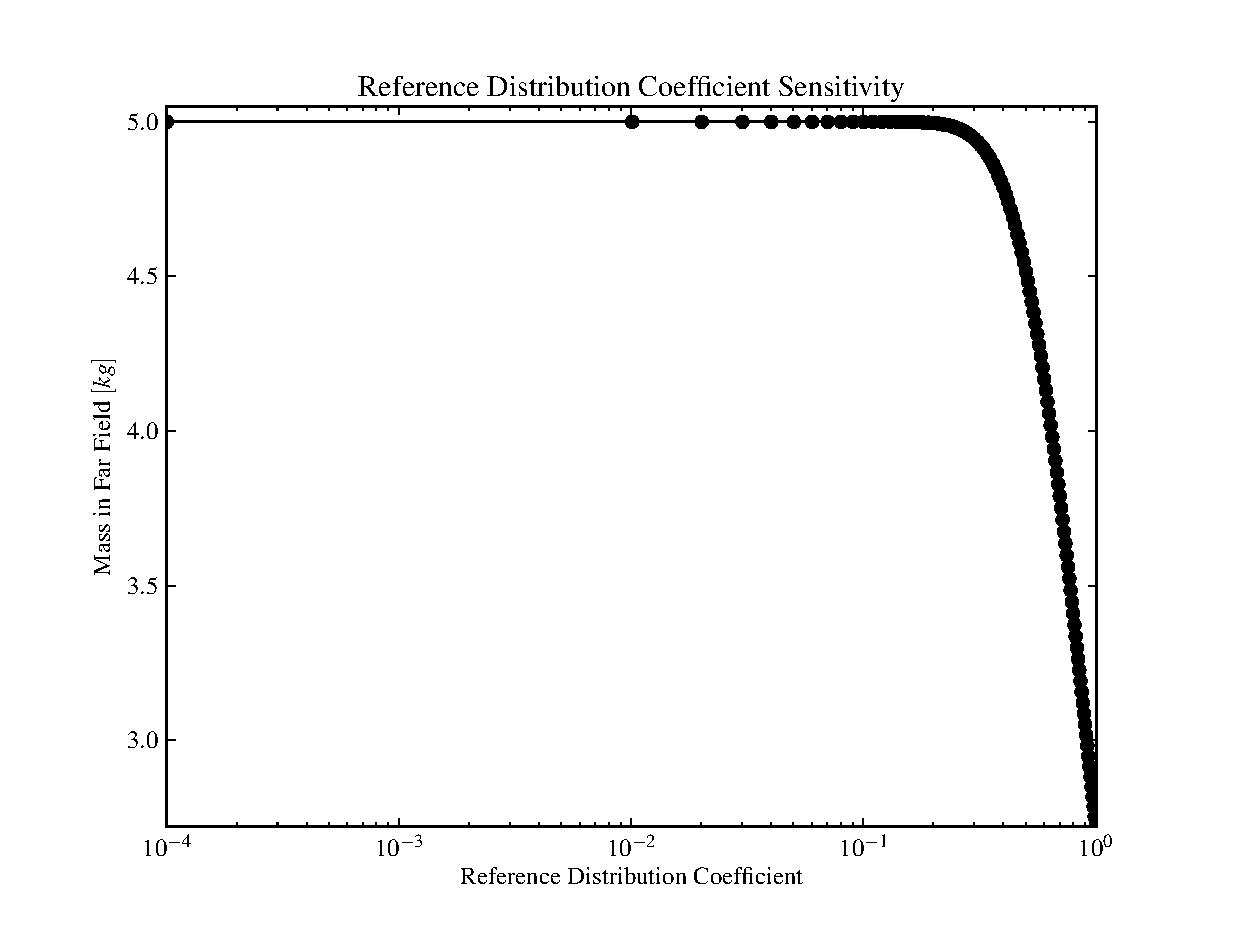
\includegraphics[width=0.7\linewidth]{./results/images/kd.eps}
\caption[$K_d$ sensitivity in the Mixed Cell Model]{$K_d$ sensitivity in the
\Cyder tool for an arbitrary isotope assigned a variable $K_d$ coefficient.}
\label{fig:kd_result}
\end{figure}


\FloatBarrier
\subsubsection{Waste Form Degradation Rate Sensitivity}
In the parametric sensitivity analysis reported in \cite{huff_key_2012}
\ref{sec:wfdeginv}, the results showed two regimes. In the first regime, the
mean of the peak annual dose rates is directly proportional to both the mass
factor (an inventory mass multiplier) and the fractional waste
form degradation rate. For some radionuclides, attenuation occurs for high
values of both parameters as the release of radionuclides is limited by
dispersion parameters. This phenomenon can be seen in the figures below in which
transition between regimes for higher degradation rates happens at lower mass
factors than transition between regimes for lower degradation rates.

The peaks for highly soluble, non-sorbing elements such as $I$ and $Cl$
are directly proportional to mass factor for most
values of waste form degradation rates. This effect can be seen in Figures
\ref{fig:WFDegI129} and \ref{fig:WFDegCl36}.


Highly soluble and non-sorbing $^{129}I$ demonstrates a direct proportionality between dose rate and
fractional degradation rate until a turnover where other natural system
parameters dampen transport.

\begin{figure}[ht!]
\begin{minipage}[b]{0.45\linewidth}
\centering
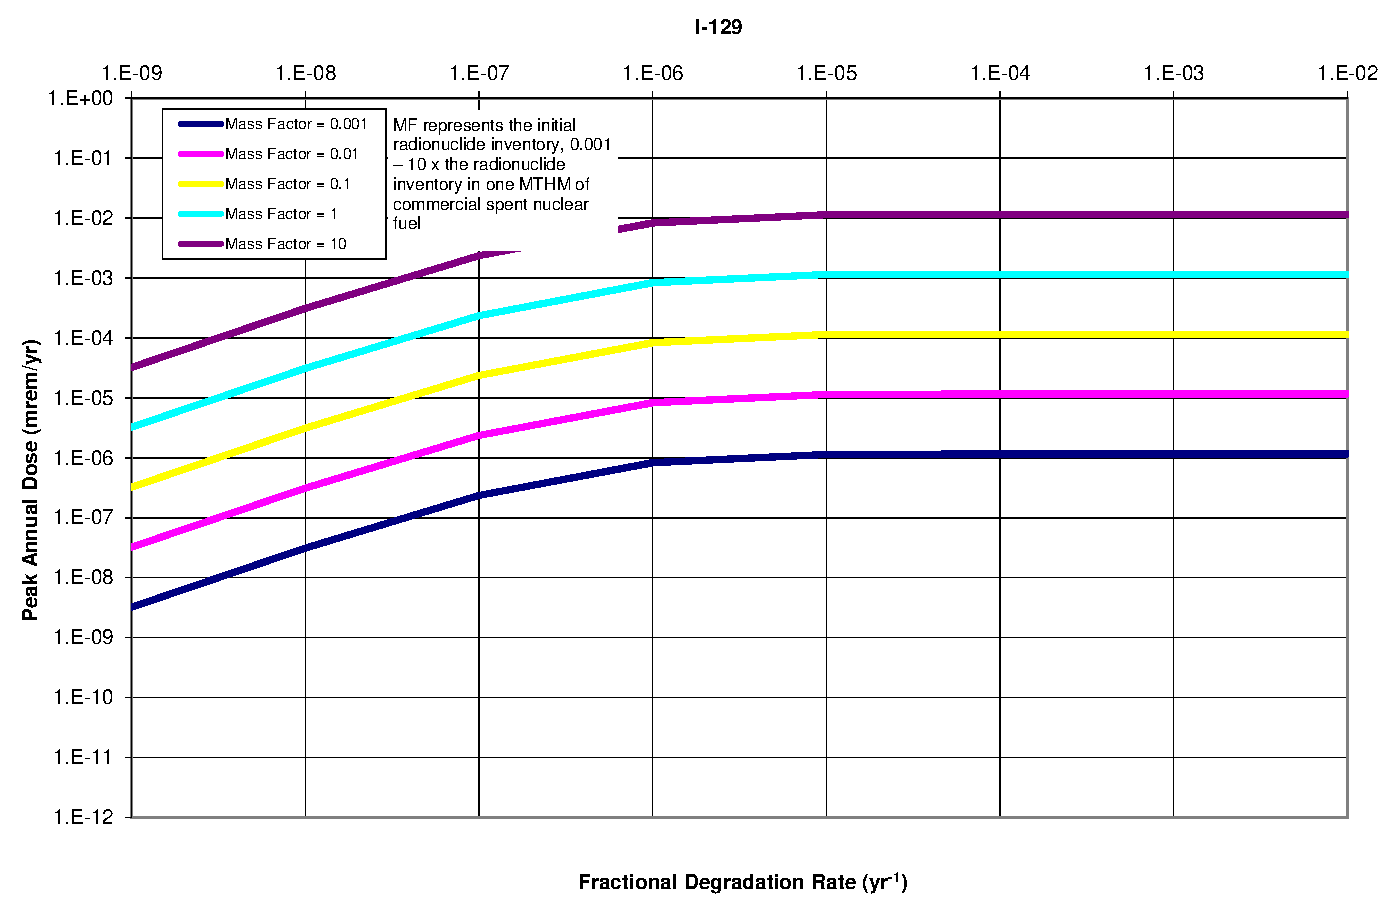
\includegraphics[width=\linewidth]{./results/images/WFDegAndInv/I-129.eps}
\caption{$^{129}I$ waste form degradation rate sensitivity.}
\label{fig:WFDegI129}

\end{minipage}
\hspace{0.05\linewidth}
\begin{minipage}[b]{0.45\linewidth}

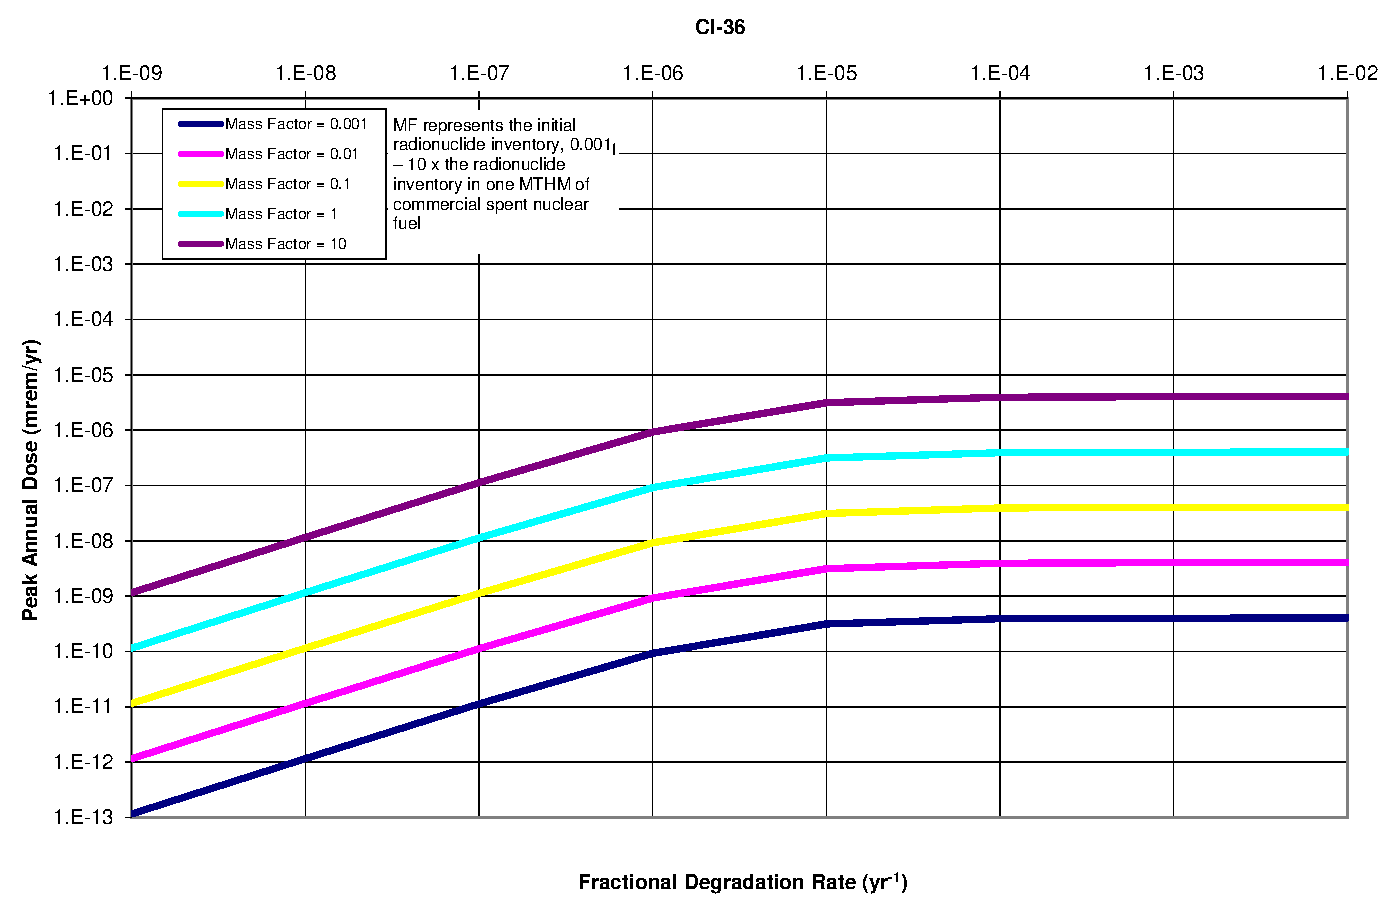
\includegraphics[width=\linewidth]{./results/images/WFDegAndInv/Cl-36.eps}
\caption{$^{36}Cl$ waste form degradation rate sensitivity.}
\label{fig:WFDegCl36}
\end{minipage}
\end{figure}

\FloatBarrier


In the parametric sensitivity analysis conducted with the \Cyder tool, waste
form degradation rate sensitvity similarly shows the two regimes noted in the
\gls{GDSM} analysis.

\begin{figure}[htbp!]
\begin{center}
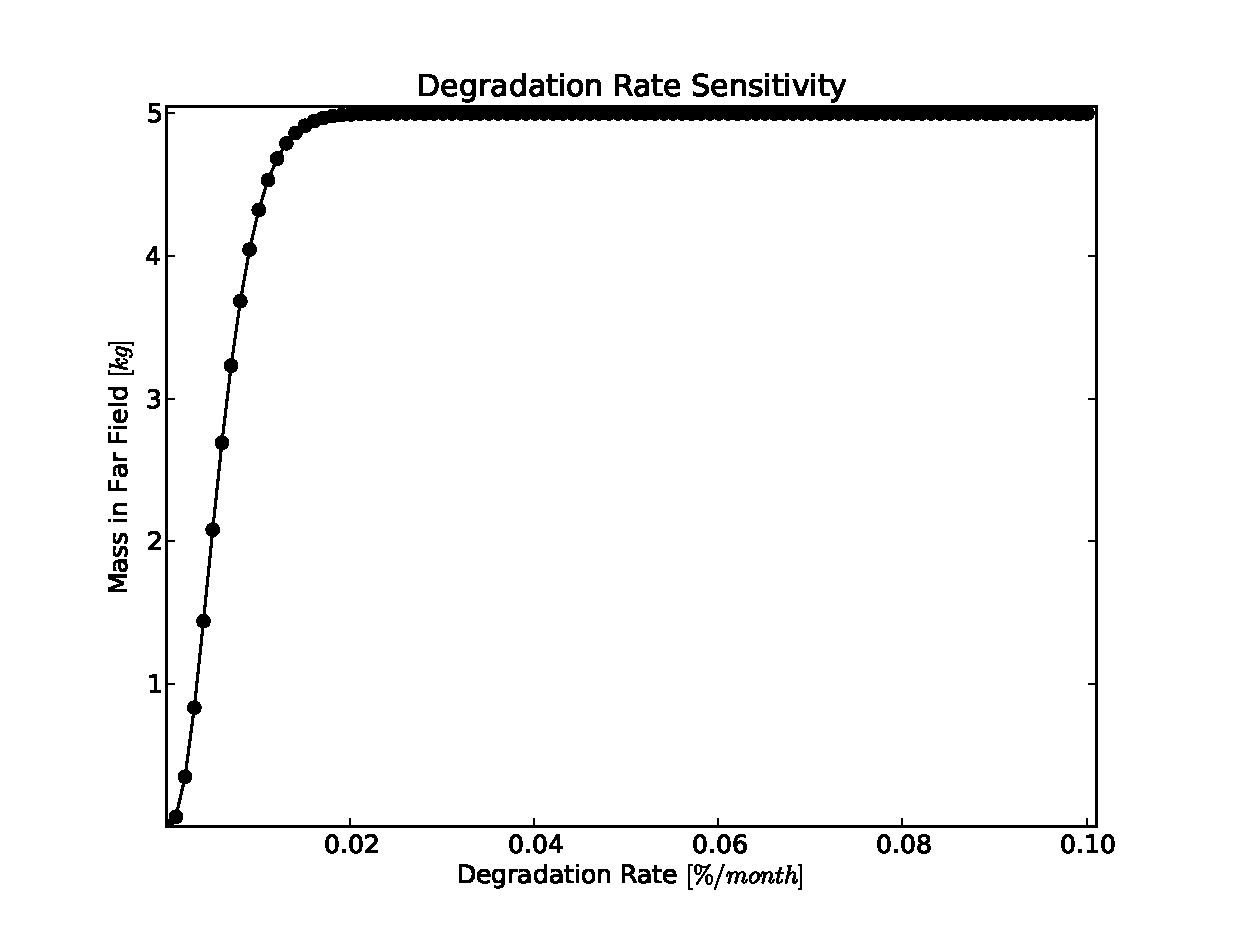
\includegraphics[width=0.7\linewidth]{./results/images/WFDegAndInv/deg.eps}
\end{center}
\caption{Sensitivity demonstration of the degradation rate in \Cyder for an
arbitrary isotope.}
\label{fig:deg}
\end{figure}


\FloatBarrier
\subsection{Significance}
% The existence of this code enables dynamic analysis of repository performance
% during fuel cycle simulation.

This work has provided a flexible code for rapid medium fidelity calculation
of generic repository performance in the context of fuel cycle analysis.
Capable of hydrologic contaminant transport discussed here, thermal transport
demonstrated elsewhere, and integration within a fuel cycle simulation code,
\Cyder is the first of its kind.

In this work, key conceptual components and modeling methods for geologic
radioactive waste disposal were identified as part of a literature review,
dominant physics of thermal and radionuclide transport were identified by
conducting sensitivity analyses with detailed codes. Accordingly, a basic set
of abstracted models were developed and implemented within the \Cyder code.

A set of basic capabilities within the \Cyder library have been developed and
validated and an assortment of advanced features, data, testing, and plotting
capabilities are functional. The \Cyder source code in which these models are
implemented is made freely available to interested researchers and potential
model developers \cite{huff_cyder_2013}. In addition to the source code and
supporting publications, the \Cyder code is well commented and produces
clickable, browsable automated documentation with each build. That
documentation is also available online \cite{huff_cyder_2013}.

The application programming interface to this software library is intentionally
general, facilitating the incorporation of the models presented here within
external software tools in need of a multicomponent disposal system simulator.

Furthermore, this work contributes to an expanding ecosystem of computational
models available for use with the Cyclus fuel cycle simulator. This hydrologic
nuclide transport library, by virtue of its capability to modularly integrate
with the Cyclus fuel cycle simulator has laid the foundation for integrated
disposal option analysis in the context of fuel cycle options.
